%%%%%%%%%%%%%%%%%%%%%%%%%%%%%%%%%%%%%%%%%%%%%%%%%%%%%%%%%%%%%%%%%%%%%
%%                                                                 %%
%% Please do not use \input{...} to include other tex files.       %%
%% Submit your LaTeX manuscript as one .tex document.              %%
%%                                                                 %%
%% All additional figures and files should be attached             %%
%% separately and not embedded in the \TeX\ document itself.       %%
%%                                                                 %%
%%%%%%%%%%%%%%%%%%%%%%%%%%%%%%%%%%%%%%%%%%%%%%%%%%%%%%%%%%%%%%%%%%%%%

%%\documentclass[referee,basic]{jnl}% referee option is meant for double line spacing

%%=======================================================%%
%% to print line numbers in the margin use lineno option %%
%%=======================================================%%

%%\documentclass[lineno,basic]{jnl}% Basic Springer Nature Reference Style/Chemistry Reference Style

%%======================================================%%
%% to compile with pdflatex/xelatex use pdflatex option %%
%%======================================================%%

%%\documentclass[pdflatex,basic]{jnl}% Basic Springer Nature Reference Style/Chemistry Reference Style

%%\documentclass[basic]{jnl}% Basic Springer Nature Reference Style/Chemistry Reference Style
\documentclass[pdflatex,mathphys]{jnl}% Math and Physical Sciences Reference Style
%%\documentclass[aps]{jnl}% American Physical Society (APS) Reference Style
%%\documentclass[vancouver]{jnl}% Vancouver Reference Style
%%\documentclass[apa]{jnl}% APA Reference Style
%%\documentclass[chicago]{jnl}% Chicago-based Humanities Reference Style
%%\documentclass[standardnature]{jnl}% Standard Nature Portfolio Reference Style
%%\documentclass[default]{jnl}% Default
%%\documentclass[default,iicol]{jnl}% Default with double column layout

\usepackage{caption}
\captionsetup{justification=justified, font=small}

%%%% Standard Packages
%%<additional latex packages if required can be included here>
%%%%

%%%%%=============================================================================%%%%
%%%%  Remarks: This template is provided to aid authors with the preparation
%%%%  of original research articles intended for submission to journals published 
%%%%  by Springer Nature. The guidance has been prepared in partnership with 
%%%%  production teams to conform to Springer Nature technical requirements. 
%%%%  Editorial and presentation requirements differ among journal portfolios and 
%%%%  research disciplines. You may find sections in this template are irrelevant 
%%%%  to your work and are empowered to omit any such section if allowed by the 
%%%%  journal you intend to submit to. The submission guidelines and policies 
%%%%  of the journal take precedence. A detailed User Manual is available in the 
%%%%  template package for technical guidance.
%%%%%=============================================================================%%%%

\jyear{2023}%

%% as per the requirement new theorem styles can be included as shown below
\theoremstyle{thmstyleone}%
\newtheorem{theorem}{Theorem}%  meant for continuous numbers
%%\newtheorem{theorem}{Theorem}[section]% meant for sectionwise numbers
%% optional argument [theorem] produces theorem numbering sequence instead of independent numbers for Proposition
\newtheorem{proposition}[theorem]{Proposition}% 
%%\newtheorem{proposition}{Proposition}% to get separate numbers for theorem and proposition etc.

\theoremstyle{thmstyletwo}%
\newtheorem{example}{Example}%
\newtheorem{remark}{Remark}%

\theoremstyle{thmstylethree}%
\newtheorem{definition}{Definition}%

\raggedbottom

\usepackage{paralist} %https://tex.stackexchange.com/questions/146306/how-to-make-horizontal-lists
%%\unnumbered% uncomment this for unnumbered level heads

\usepackage{siunitx} %https://tex.stackexchange.com/questions/2746/aligning-numbers-by-decimal-points-in-table-columns

\begin{document}

\title[Building pangenome graphs]{Building pangenome graphs}

%%=============================================================%%
%% Prefix	-> \pfx{Dr}
%% GivenName	-> \fnm{Joergen W.}
%% Particle	-> \spfx{van der} -> surname prefix
%% FamilyName	-> \sur{Ploeg}
%% Suffix	-> \sfx{IV}
%% NatureName	-> \tanm{Poet Laureate} -> Title after name
%% Degrees	-> \dgr{MSc, PhD}
%% \author*[1,2]{\pfx{Dr} \fnm{Joergen W.} \spfx{van der} \sur{Ploeg} \sfx{IV} \tanm{Poet Laureate} 
%%                 \dgr{MSc, PhD}}\email{iauthor@gmail.com}
%%=============================================================%%

\author*[1]{\fnm{Erik} \sur{Garrison}}\email{egarris5@uthsc.edu}
\equalcont{These authors contributed equally to this work.}
\author[1,2]{\fnm{Andrea} \sur{Guarracino}}
\equalcont{These authors contributed equally to this work.}
\author[3,4]{\fnm{Simon} \sur{Heumos}}
\author[1]{\fnm{Flavia} \sur{Villani}}
\author[5]{\fnm{Zhigui} \sur{Bao}}
\author[6]{\fnm{Lorenzo} \sur{Tattini}}
\author[7]{\fnm{J\"{o}rg} \sur{Hagmann}}
\author[8]{\fnm{Sebastian} \sur{Vorbrugg}}
\author[9,10]{\fnm{Santiago} \sur{Marco-Sola}}
\author[8]{\fnm{Christian} \sur{Kubica}}
\author[1]{\fnm{David G.} \sur{Ashbrook}}
\author[11]{\fnm{Kaisa} \sur{Thorell}\textsuperscript{11}}
\author[12]{\fnm{Rachel L.} \sur{Rusholme-Pilcher}}
\author[6]{\fnm{Gianni} \sur{Liti}}
\author[13]{\fnm{Emilio} \sur{Rudbeck}}
\author[14]{\fnm{Agnieszka A.} \sur{Golicz}}
\author[3,4]{\fnm{Sven} \sur{Nahnsen}}
\author[15]{\fnm{Zuyu} \sur{Yang}}
\author[16]{\fnm{Moses N.} \sur{Mwaniki}}
\author[17]{\fnm{Franklin L.} \sur{Nobrega}}
\author[17]{\fnm{Yi} \sur{Wu}}
\author[18]{\fnm{Hao} \sur{Chen}}
\author[15]{\fnm{Joep} \sur{de Ligt}}
\author[19]{\fnm{Peter H.} \sur{Sudmant}}
\author[20,21,22,23,2]{\fnm{Nicole} \sur{Soranzo}}
\author[1,24]{\fnm{Vincenza} \sur{Colonna}}
\author[1]{\fnm{Robert W.} \sur{Williams}}
\author[1]{\fnm{Pjotr} \sur{Prins}}

\affil[1]{Department of Genetics, Genomics and Informatics, University of Tennessee Health Science Center, 71 S Manassas St, Memphis, 38163, Tennessee, USA}
\affil[2]{Fondazione Human Technopole, Viale Rita Levi Montalcini, 20157 Milan, Italy}
\affil[3]{Quantitative Biology Center (QBiC) T\"{u}bingen, University of T\"{u}bingen, T\"{u}bingen, Germany}
\affil[4]{Biomedical Data Science, Dept. of Computer Science, University of T\"{u}bingen, T\"{u}bingen, Germany}
\affil[5]{Shenzhen Branch, Guangdong Laboratory of Lingnan Modern Agriculture, Genome Analysis Laboratory of the Ministry of Agriculture and Rural Affairs, Agricultural Genomics Institute at Shenzhen, Chinese Academy of Agricultural Sciences, Buxin Road 97, Shenzhen, 518120, Guangdong, China}
\affil[6]{Universit\'{e} C\^{o}te d'Azur, CNRS, INSERM, IRCAN, Nice, France}
\affil[7]{Computomics GmbH, Eisenbahnstr. 1, 72072 T\"{u}bingen, Germany}
\affil[8]{Department of Molecular Biology, Max Planck Institute for Biology, Max-Planck-Ring 9, 72076 T\"{u}bingen, Baden-Wuerttemberg, Germany}
\affil[9]{Computer Sciences Department, Barcelona Supercomputing Center, Barcelona 08034, Spain}
\affil[10]{Departament d'Arquitectura de Computadors i Sistemes Operatius, Universitat Autonoma de Barcelona, Barcelona 08193, Spain}
\affil[11]{Chemistry and Molecular Biology, Faculty of Science, University of Gothenburg, Sweden}
\affil[12]{Earlham Institute, Norwich Research Park, Colney Lane, Norwich, Norfolk, NR4 7UZ. UK}
\affil[13]{Clinical Genomics Gothenburg, Bioinformatics and Data Centre, University of Gothenburg, Sweden}
\affil[14]{Department of Plant Breeding, Justus Liebig University Giessen, Giessen, Germany}
\affil[15]{The Institute of Environmental Science and Research, New Zealand}
\affil[16]{Department of Computer Science, University of Pisa}
\affil[17]{School of Biological Sciences, Faculty of Environmental and Life Sciences, University of Southampton, Southampton, UK}
\affil[18]{Department of Pharmacology, Addiction Science and Toxicology, University of Tennessee Health Science Center, Memphis, TN}
\affil[19]{Department of Integrative Biology, University of California Berkeley, Berkeley, CA}
\affil[20]{Wellcome Sanger Institute, Genome Campus, Hinxton CB10 1SA, UK}
\affil[21]{National Institute for Health Research Blood and Transplant Research Unit in Donor Health and Genomics, University of Cambridge, Cambridge, UK}
\affil[22]{Department of Haematology, Cambridge Biomedical Campus, Cambridge CB2 0AW, UK}
\affil[23]{British Heart Foundation Centre of Research Excellence, University of Cambridge, Cambridge, UK}
\affil[24]{Institute of Genetics and Biophysics, National Research Council, Naples 80111, Italy}




%%==================================%%
%% sample for unstructured abstract %%
%%==================================%%

%\abstract{
%The PanGenome Graph Builder (PGGB) is a reference-free pangenome graph construction pipeline to better represent and analyze multiple genomes.
%Unlike existing approaches that are reference-guided, PGGB computes all-to-all genome-wide alignments to build a variation graph.
%Through iterative graph embedding, partitioning, and local reconstruction, PGGB builds a pangenome graph that can be used to detect variation, measure conservation, detect recombination events, and infer phylogenetic relationships.
%}

%\abstract{
%  The PanGenome Graph Builder (PGGB) is a reference-free method to represent and analyze multiple genomes. It computes genome-wide alignments for each genome pair and builds an unbiased, accurate pangenome graph that can detect variation, measure conservation, detect recombination events, and infer phylogenetic relationships. PGGB is applied to diverse species, providing an efficient and reliable tool for sequence evolution and variation analysis.
%  }

\abstract{
  Pangenome graphs can represent all variation between multiple genomes, but existing methods for constructing them are biased due to reference-guided approaches.
  In response, we developed the PanGenome Graph Builder (PGGB), a reference-free pipeline for constructing unbiased pangenome graphs.
  PGGB uses all-to-all whole-genome alignments and learned graph embeddings to build and iteratively refine a model in which we can identify variation, measure conservation, detect recombination events, and infer phylogenetic relationships.
  %, providing an efficient and unbiased tool for studying sequence evolution and variation in diverse species.
}

%\abstract{
%  The PanGenome Graph Builder (PGGB) is a reference-free pangenome graph construction pipeline that proposes a symmetric approach to represent and analyze multiple genomes.
%  Unlike existing approaches that are reference-guided, PGGB computes all-to-all genome-wide alignments for each genome pair in the dataset to build a variation graph.
%  Through iterative graph embedding, partitioning, and local reconstruction, PGGB builds an unbiased and accurate pangenome graph that can be used to detect variation, measure conservation, detect recombination events, and infer phylogenetic relationships in diverse species from across the tree of life.
%  }

%\abstract{
%  Pangenome graphs provide an efficient model to represent and analyze multiple genomes.
%  Existing approaches to build them are reference-guided, which leads to bias that can affect downstream applications.
%  In response, we propose the PanGenome Graph Builder (PGGB), a symmetric, reference-free pangenome graph construction pipeline.
%  PGGB first computes all-to-all genome-wide alignments for each genome pair in the dataset.
%  It converts these to a variation graph, which is refined through iterative graph embedding, partitioning, and local reconstruction.
%  The built pangenome graph may then be used to identify variation, measure conservation, detect recombination events, and infer phylogenetic relationships.
%  We apply PGGB to diverse species from across the tree of life, and show that it provides unbiased, accurate interpretations of sequence evolution and variation.
%}

\keywords{pangenomes, genome alignment, variant detection, comparative genomics, chromosome evolution, phylogenetics, population genetics}
%%\pacs[JEL Classification]{D8, H51}

%%\pacs[MSC Classification]{35A01, 65L10, 65L12, 65L20, 65L70}

\maketitle

Pangenome graphs compactly represent complete genomes, their homologies, and all forms of variation between them \cite{Garrison_2018,Paten_2017,Garrison_2019,Eizenga2020}.
They allow us to identify variation, measure conservation, detect recombination events, and infer phylogenetic relationships, making them valuable tools for studying sequence evolution and variation in diverse species \cite{Armstrong2020,Guarracino_odgi_2022}.
However, existing methods for constructing pangenome graphs \cite{Li2020,Hickey_2023} are biased due to their reference and tree-guided approaches \cite{Armstrong2020,Noll_2022}, which can lead to incomplete and unstable representations of genetic variation \cite{Garrison_seqwish_2022}.
Inductive biases result from techniques to mitigate computational complexity \cite{Li2020,Armstrong2020}, or from a goal to structure the resulting graphs so that they are easier to use during read alignment \cite{Hickey_2023}.
The unbiased construction of pangenome graphs implies all-to-all comparisons that scale quadratically with the number of included genomes \cite{Garrison_seqwish_2022}.
Although approaches for unbiased pangenome graph construction have been proposed \cite{Minkin_2016,Garrison_seqwish_2022}, these have been limited to the graph induction step, and specialized techniques for pangenome alignment and refinement are required to avoid systematic biases and obtain high-quality pangenome builds \cite{Liao_2023}.

\begin{figure}[htbp!]
%    \centering
	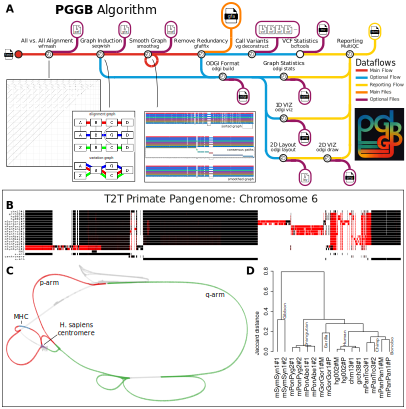
\includegraphics[width=\linewidth]{fig/figure1.pdf}
	\caption{
      \textbf{PGGB and applications.}
      (A) PGGB’s algorithms/data flows.
      Primary flow (red) proceeds from FASTA to alignment, graph induction, smoothing, to normalization with GFAF-FIX, ending with final graph (orange). Optional outputs (blue): statistics, variant calls, and 1D/2D graph visualizations.
      (B) 1D pangenome graph visualization using 14 haplotype-resolved primate assemblies homologous to human chromosome 6.
      T2T-CHM13 annotations (Major Histocompatibility Complex, p-arm, centromere, q-arm) are shown.
      The p-arm region with the MHC is inverted in Gibbon.
      Centromeric regions appear largely non-homologous among many species, with the exception of between chimpanzee and bonobo and between the orangutans.
      (C) 2D visualization, rendered with the same human chromosomal annotations in GFAESTUS \cite{Fischer_2022}, shows possible circularization due to structural variation or homogenization between subtelomeric regions.
      (D) Using ODGI \cite{Guarracino_odgi_2022}, we extract a pairwise distance matrix based on in-graph Jaccard metrics over shared base pairs.
      This distance matrix yields a phylogenetic tree that matches previous results based on SNPs \cite{Cagan_2016}.
      We posit that the greater phylogenetic distances reflect the inclusion of the centromeres---which feature low rates of recombination and tend to diversify rapidly by near-clonal evolution \cite{Logsdon2021}---in our distance computation.
    }
	\label{fig:pggb}
\end{figure}

To overcome these limitations, we propose the PanGenome Graph Builder (PGGB), a reference-free pipeline to construct unbiased pangenome graphs.
%PGGB is the first whole genome alignment or pangenome construction method to achieve diverse goals.
Its output presents a base-level representation of the pangenome, including variants of all scales from single nucleotide polymorphisms (SNPs) to structural variants (SVs).
The graph is unbiased, i.e., all genomes are treated equivalently, regardless of input order or phylogenetic dependencies, and any genome may be used as a frame of reference in downstream analysis.
PGGB makes no assumptions about phylogenetic relationships, orthology groups, or evolutionary histories, allowing data to speak for itself without risks of implicit biases that may affect inferences made from the graph.
PGGB is implemented as a modular shell script, integrating independent components via standard text-based file formats, which provides a template for future pangenome construction methods.
The method is practical, scalable to hundreds of genomes, and has been proven accurate through years of development in the Human Pangenome Reference Consortium (HPRC) \cite{Liao_2023,Guarracino_2023} and in the broader bioinformatics community \cite{crysnanto2022comparison,zhang2022fast,Leonard_2022,Zhou_2022}.
Here, we describe the specific innovations in the three main phases of the algorithm: alignment, graph creation, and graph normalization.
We then use cross-validation with MUMMER4 \cite{Marcais_2018} to demonstrate the accuracy of our approach across a wide range of species and scales.

PGGB begins with sequence alignment (Figure \ref{fig:pggb}A).
%Although any input alignments may be used, 
To avoid reference and order bias, PGGB uses an all-to-all alignment of the input sequences.
This approach aligns sequences directly to each other, enabling each sequence in the pangenome to serve as a potential reference to describe variation.
To obtain alignments, PGGB uses WFMASH \cite{Guarracino_wfmash_2021}.
WFMASH first applies an extension of MASHMAP \cite{Jain_2018} to obtain high-level homology mappings, by default using seeds of 5kbp to find homologies of 25kbp or more at 90\% average nucleotide identity.
%MASHMAP provides highly efficient, accurate detection of homologies among genomes \cite{Jain_2018} and even across whole pangenomes \cite{Guarracino_2023}.
WFMASH then uses a generalization of the bidirectional Wavefront Algorithm (BiWFA) \cite{Marco_Sola_2020,Marco_Sola_2023} that aligns the sequences by comparing segments of 256bp rather than single characters.
This algorithm, BiWF$\lambda$---so named because it replaces character match with a callback function $\lambda$ that matches segments---obtains a final base level alignment by splicing together ``incepted'' alignments over the 256bp segment pairs that lie in the optimal alignment path.
Our use of WFMASH ensures that the alignments which structure the graph feature long-range collinearity that is insensitive to repetitive, shorter homologies found between transposons and satellite sequences.
Although WFMASH alignments have an ideal structure for its operation, PGGB can build the graph using any set of user-defined alignments in PAF format.
%However, the use of WFMASH is not specifically required, and PGGB supports the use of any user-defined input alignment set in PAF format.

The second step---pangenome graph induction---converts a collection of genomes and pairwise alignments between them into an equivalent variation graph.
We achieve this with SEQWISH \cite{Garrison_seqwish_2022}, a tool specifically designed to scale graph induction to whole pangenomes in low memory.
At a high level, SEQWISH merges all DNA base-pairs that are matched together in the alignments into a single character in the output graph.
This process also compresses transitively-matched base-pairs.
For example, if $A$, $B$, and $C$ are characters in input sequences and $\to$ represents a character match, $A \to B \to C$ would result in a single character in the output graph that also implies the transitive match $A \to C$.
SEQWISH evokes this transitive closure while retaining the mapping between input sequences and the output graph, allowing it to losslessly embed the input sequences as paths through the resulting graph.
Any single input genome is faithfully and fully embedded in the graph and can be completely extracted by tracing labeled paths through the nodes.
The SEQWISH graph thus recovers transitive homology relationships that may not be present in the initial alignment set.
This property allows us to apply random sparsification to reduce the complexity of very large alignment problems.

For large inputs, PGGB can use a heuristic based on the Erdős–Rényi model of random graphs to set a sparsification threshold for initial mappings.
This model leads us to expect a giant component, or connected subgraph that contains a significant portion of the nodes in the graph, to arise in a random graph of $N$ nodes when the probability of edges between two nodes is $P_{critical}=1/(N-1)$ \cite{bollobas2001evolution}.
%If each contig is a node and edges represent mappings, then we seek a subset of mappings that ensures that we can recover homologies through transitive relationships without needing to compute all possible pairwise mappings. %---in other words, we hope to generate a giant component for every region of the pangenome graph.
Considering the SEQWISH alignment graph (Figure \ref{fig:pggb}A), where nodes correspond to subsequences and edges to mappings, we seek to ensure that a giant component exists for all homologous collections of nodes in all regions of the pangenome.
This will let us reconstruct all transitive relationships in the variation graph without needing to directly compute all pairwise alignments.
%This corresponds to a giant component connecting all genomes at each part of the SEQWISH alignment graph.
We thus set a sparsification parameter that uses a hash of each mapping record to filter mappings with a probability $P_{sparse} \gg P_{critical}$, allowing us to avoid the expected $O(N^2)$ costs implied when $P=1$.
%Our intuition is that, if the graph is based on homologous genomes, we expect all possible pairs of mappings between contigs to be valid, but the vast majority will be redundant, and discoverable via transitive relationships in the alignment graph processed by SEQWISH.
This allows us to dramatically reduce the runtime of alignment and graph induction with negligible effect on accuracy (Table~\ref{tab:table1}), e.g. $10\times$ increase in the number of genomes requires only $20\times$ increase in runtime---rather than $100\times$.
%, e.g. with sparsification we pay 1/5th the expected costs for a 10-fold increase in \textit{E. coli} genomes.
%, e.g. using sparsification for \textit{E. coli} a 10-fold increase in genomes requires only a 20-fold increase in runtime.
%for instance for \textit{E. coli} we require only $\approx 20\times$ the runtime for a 10-fold increase in genomes, while without sparsification we would expect a $100\times$ increase.

\begin{table}[b] %[ht!]
%  \centering
  \setlength{\tabcolsep}{3pt}
    {%\footnotesize
\begin{tabular}{
l
r
S[table-number-alignment = center]
S[table-number-alignment = center]
S[table-number-alignment = center]
r
l}
\multicolumn{1}{c}{\textbf{Pangenome}} & \textbf{Size (bp)} & \textbf{Compr.} & \textbf{Time (m)} & \textbf{Mem. (GB)} & \textbf{SNVs} & \textbf{F-score} \\
athaliana7.chr1 & 210174177 & 5.12 & 28.51 & 9.71 & 129374 & 0.877267 \\
ecoli50 & 249520474 & 12.56 & 89.35 & 12.97 & 56915 & 0.947041 \\
ecoli500* & 2572341327 & 23.99 & 1816.66 & 134.59 & 58259 & 0.936551 \\
hsapiens90.chr6 & 15508376475 & 81.17 & 1183.33 & 135.52 & 143972 & 0.971475 \\
mouse17.chr19 & 994731502 & 11.52 & 203.80 & 29.48 & 223951 & 0.907288 \\
primate14.chr6 & 2635610277 & 6.18 & 1742.37 & 61.38 & 2886064 & 0.909077 \\
scerevisiae8 & 96255507 & 6.47 & 8.78 & 3.53 & 53742 & 0.968729 \\
scerevisiae142 & 1702093905 & 55.29 & 1021.81 & 112.98 & 62796 & 0.955988 \\
scerevisiae142* & 1702093905 & 41.41 & 562.89 & 75.91 & 62580 & 0.955650 \\
soy37.chr18 & 2240871558 & 20.50 & 599.66 & 29.17 & 101907 & 0.907878 \\
tomato23.chr2 & 1280460312 & 20.69 & 78.53 & 43.84 & 39243 & 0.948173 \\
\\
\end{tabular}
}
    \caption{\textbf{Performance of PGGB with pangenomes across species.} \\For each pangenome, we report its size, the compression ratio (pangenome sequence length divided by graph size), the PGGB runtime, the maximum memory usage of PGGB, the average number of SNVs (across all haplotypes except the one used as reference) identified with MUMMER4 that we used to evaluate SNVs identified with PGGB, and the average F-score (across all haplotypes except the one used as reference) computed using MUMMER4's SNVs as ground truth. The name of each pangenome indicates the species and the number of haplotypes. All runs were performed on machines equipped with AMD EPYC 7402P 24-Core, 378 GB of RAM, and a 1 TB Solid-State Drive. All PGGB runs were executed with 48 threads. *Erdős–Rényi random sparsification activated.}
     \label{tab:table1}
\end{table}

Graph building completes with SMOOTHXG (Figure \ref{fig:pggb}A), an iterative post-processing step specifically designed for PGGB that locally compresses and simplifies the pangenome graph.
Although the SEQWISH graph presents a complete, lossless model of the input genomes and their homologies, in our experience it often presents complex local motifs that can cause problems for diverse types of downstream analysis.
A key issue is that pairwise alignments derived across input sequences are not mutually normalized, leading to different representations of small variants like indels in low-complexity sequences, which in turn generate complex looping motifs that are difficult to process.
We mitigate this issue by removing short matches from SEQWISH's input alignments.
This reduces complexity, but also creates a graph that can be locally ``under-aligned'' and does not represent all local pairwise relationships.
To resolve this, we apply a local realignment kernel, partial order alignment (POA) \cite{Lee2002,Vaser_2017,Gao_2020}, across all parts of the graph.
By default, we do so at a scale of around 1kbp, which is smaller than most nonlinear patterns of structural variation found in genomes \cite{Liao_2023,Vollger_2023}.
%This scale is configurable depending on the specifics of the species under study.
This allows the PGGB graph to represent complex structurally-variable loci as simple loops through a single copy of duplicated sequences \cite{Liao_2023}.
The kernel is applied to regions that are extracted from a 1-dimensional graph embedding \cite{Guarracino_odgi_2022}.
This embedding orders nodes in the graph so that their distance in the order best-approximates their distance in the genomic paths of the graph.
SMOOTHXG first learns this embedding, then obtains partially overlapping segments of the graph (blocks) to which it then applies POA.
The realigned blocks are ``laced'' back into a complete variation graph.
We iterate the entire SMOOTHXG step multiple times (3 by default) to limit edge effects that can occur near block boundaries, progressively refining the learned graph embedding.
As a final normalization step, we apply GFAFFIX to compress redundant nodes \cite{Doerr_2023} and use ODGI to make a final sort for the modified graph \cite{Guarracino_odgi_2022}.

%Downstream applications of pangenome graphs are diverse (Figure \ref{fig:pggb}A).
PGGB provides outputs that support immediate interpretation, quality control, and downstream applications.
%PGGB integrates common steps that help to provide immediate feedback on graph build quality.
Using ODGI, it produces basic graph statistics, such as size, node count, and base content.
ODGI creates 1D and 2D visualizations that provide intuition about the structure of the entire graph, with the 1D view showing the relative alignment of paths into the graph structure, and the 2D view showing high-level features of the graph topology.
Both can be applied at the scale of multi-gigabasepair graphs.
Optionally, PGGB provides graph statistics and diagnostic plots in a MultiQC report \cite{Ewels2016}.
We also provide an option to call variants \cite{Garrison_2018,Paten_2018} from the graph to produce a phased description of embedded haplotypes in variant call format (VCF).
Variants called directly from the graph can include large nested genetic sites, leading to incompatibility with many applications.
To address this, PGGB decomposes complex nested variation into a minimal reference-relative representation using BiWFA \cite{Garrison_vcflib_2022}.
This allows PGGB to provide input to analyses based on small variants, leading to compatibility with numerous downstream applications based on genomic variation.
PGGB is thus a multi-sample variant caller for whole-genome assemblies.

PGGB has been applied and validated at large scale in projects in the HPRC \cite{Liao_2023}, where it additionally has provided the first sequence-based evidence for systematic recombination between heterologous acrocentric human chromosomes \cite{Guarracino_2023}.
Here, to demonstrate PGGB's broad utility, we present results from its application to a variety of diverse pangenome and comparative genomic contexts (Table~\ref{tab:table1}).
We provide information on runtime and resource requirements, showing that even for hundreds of small genomes, PGGB can provide a variation graph within hours.
Larger genomes in general require partitioning to maximize parallelism and ensure that total compute requirements fit in standard commodity servers (Section \ref{sec:partition}).
Due to lack of ground truth, quality evaluation on real data can be difficult.
For validation, we compare PGGB's output with SNPs detected by MUMMER4 \cite{Marcais_2018}, a current standard approach for pairwise whole genome alignment.
These show cross validation F-scores $>$90\% across all tested contexts except \textit{athaliana7.chr1}, indicating that the method performs equivalently to existing standards.
However, while MUMMER4 provides only pairwise comparisons with a target reference, PGGB yields a full all-to-all comparison between genomes that leads to completely new bioinformatic analysis modalities.

%As a demonstration of the transformative utility of our approach,
Many downstream applications that are typically based on polarization of variants (e.g. SNPs) relative to a single reference genome may be directly implemented in the space of variation graphs built with PGGB and similar methods. % and related methods.
This follows from two basic concepts: in the variation graph, nodes are alleles, while genomes can be simply understood as vectors of allele counts.
Methods based in this vector space allow us to simultaneously consider \emph{all} classes of variation in downstream analyses, without reference bias, an objective, which to our knowledge has never been achieved before in bioinformatics with the practical generality provided by PGGB.
As proof of principle, we put forward a phylogenetic tree constructed directly from distances measured within a pangenome graph of 14 complete assemblies of chromosome six from the great ape family (Figure \ref{fig:pggb}D), which matches established phylogenies of the \textit{Hominoidea} clade based on manually curated sets of SNPs that exclude structurally variable regions \cite{Cagan_2016}.

%In summary,
PGGB is a new, modular, and conceptually straightforward approach to understanding sequence relationships between many complete genomes in both pangenomic and comparative genomics settings.
Our approach provides a general framework for genome graph building techniques which we expect researchers will upgrade and extend in the future.
By making it easy to build variation graphs, PGGB opens the door to diverse downstream population and evolutionary genetic methods that can consider all classes of sequence variation simultaneously.
This will allow us to develop a comprehensive understanding of the links between sequence variation, phenotype, and evolution in an era where the complete assembly of genomes becomes routine.

%This step removes the reference bias from pangenome analysis, leading to an unbiased representation of genetic variation.


%New assembly approaches based on high-accuracy long sequence reads enabled the assembly of regions of the genomes that were previously inaccessible~\cite{Nurk2021, Logsdon2021, Ebert2021}.
%The study of all these high-quality assemblies has therefore opened the door for a comprehensive understanding of the genomic variability of populations.
%Pangenomes are models able to fully represent collections of sequences and their variation~\cite{Eizenga2020}.
%A standard model for this representation is the pangenome graph, where similar orthologous regions between genomes collapse into a single representative sequence.
%This sequence graph model relates the sequences in a pangenome to each other by encoding them as walks through a common underlying sequence graph.
%When built from comprehensive, accurate alignments, pangenome graphs allow us to understand all genetic variation between all sequences in the pangenome.

%However, pangenome building is an open problem.
%To properly understand genome variability and evolution, we need to obtain an unbiased image of the relationship between multiple sequences.
%Due to the quadratic scaling of the all-to-all problem, researchers have instead focused on progressively building the alignment,
%starting with the reference~\cite{Li2020} or using a phylogenetic guide tree to limit the number of alignments~\cite{Armstrong2020}.
%These approaches introduce bias into the resulting model.
%By definition, a progressive approach will generate different structures depending on the order in which genomes are included~\cite{Lee2002, Grasso2004}.
%Moreover, its resulting representation, with a linear reference and a hierarchy of structural variation build out of it,
%is inappropriate for representing large scale features present in general pangenome graphs~\cite{Sekar2016, Hollox2008, Vollger2021},
%as structural and evolutionary-scale variation do not respect the simplistic linear and hierarchical model.
%To date, it has been approached by using alignment methods that were traditionally used for large multiple sequence alignments, such as partial order alignment (POA)\cite{Lee2002}.
%Minigraph~\cite{Li2020} applies a POA-based generalization of the Minimap2~\cite{Li2018} minimizer chaining algorithm to sequence directed acyclic graphs (DAGs).
%This produces a simple DAG, with a linear reference and a hierarchy of structural variation build out of it.
%A guide tree has sense when considering distantly-related groups, but it breaks down within species or in the case of incomplete lineage sorting,
%such as is found in the human and primate MHC~\cite{Scally2012}.
%Therefore, when using these alignment methods, the detected structure of variation depends on the chose reference, order, and guide tree.
%Furthermore, to apply such approaches, researchers had to mask new satellite sequences, as well as newly assembled regions on the acrocentric p-arms [FIXME CITATION NEEDED].
%fixme other pangenome building pipelines in the introduction?
%We believe that it is necessary to establish methods that can handle all genomic sequences, including complex regions and their putatively nonlinear patterns of variation.

%To overcome the limitations of current pangenome building approaches, we implemented the PanGenome Graph Builder (PGGB) pipeline (Fig.~\ref{fig:pggb}). %(\hyperref[fig:pggb]{Fig. 1}). https://tex.stackexchange.com/questions/378107/ref-to-a-label-with-a-new-link-name
%PGGB renders a collection of sequences into a variation graph~\cite{Garrison2018} able to represent any kind of relationships between them.
%Such a pangenome graph is locally directed and acyclic while preserving large-scale variation.
%Maintaining local linearity is important for pangenome graphs visualization and interpretation.
%PGGB consists of three main steps, i.e. sequence alignment, graph construction, and graph normalization, but our approach is modular and flexible.
%This means that any step can be modified, or replaced by other tools, without affecting the others.

%\input{fig_pggb.tex}

%The equal treatment of all genomes is critical to build a pangenome which provides an equitable foundation for studies of genome variation and evolution.
%To avoid reference and order bias, the first step in PGGB is the all-to-all alignment of the input sequences.
%We apply WFMASH~\cite{Guarracino_wfmash_2021}, an alignment algorithm that supports rapid and accurate pairwise alignment of T2T assemblies.
%Our approach is fundamentally trivial: we align the sequences directly to each other.
%Each sequence in a pangenome is thus a potential reference for understanding all related variation.
%This allows us to remove the reference bias from pangenome analysis.
%The all-to-all alignment of genomes embeds their pluralistic homologies and it implies a variation graph.
%The second step in PGGB is to losslessly convert the alignments into the variation graph model.
%We apply SEQWISH~\cite{Garrison2022}, a tool that renders a variation graph from a set of input sequences and alignments between them.
%Like the alignment method we apply, this construction method leads to an unbiased pangenome graph.
%Nevertheless, pangenome graphs produced directly from pairwise alignments contain very complex local structures that result from ambiguous alignments between repetitive sequences.
%This issue is akin to the \textit{indel realignment problem} faced during the processing of Illumina sequencing data~\cite{Mose2019}.
%To mitigate this issue, and to improve process efficiency, we typically build our initial raw pangenome graph after
%filtering the alignments to preserve matches longer than a fixed threshold.
%In result, the graph may also be locally underaligned.
%While the large-scale structure of the graph is correct, the base-level alignments suffer from the erosion of the small matches in the alignments.
%These issues led us to implement a third step in PGGB for pangenome graph normalization.
%Although structural variation (SV) adds nonlinear complexity to the full pangenome graph, because DNA sequences are linear, in
%any local context of the pangenome their relationships tend to be represented in a linear, ordered model like a multiple sequence alignment.
%We enforce this prior intuition by applying SMOOTHXG (SUPP. METHODS FOR ITS EXPLANATION, SUPP. Fig.~\ref{fig:smoothxg}), a tool that normalizes the
%graph in one or multiple steps by running a partial order alignment (POA)~\cite{Lee2002} algorithm over small pieces of the graph, letting larger SVs remain nonlinear.
%Finally, the normalized pangenome graph is processed by GFAFFIX (CITE https://github.com/marschall-lab/GFAffix), a tool to identify and collapse redundant structures in the graph.
%PGGB concludes with tools that generate vital graph statistics, 1D, and 2D visualizations of the graph and its embedded paths using the graph genome toolkit ODGI~\cite{Guarracino2022}. All diagnostic output is aggregated in a MultiQC~\cite{Ewels2016} report.
%Futhermore, PGGB can optionally generate a multiple sequence alignment in the traditional MAF format, and VCF files against any chosen set of reference sequences embedded in the pangenome graph.

%The Introduction section, of referenced text \cite{bib1} expands on the background of the work (some overlap with the Abstract is acceptable).
%The introduction should not include subheadings.

%Springer Nature does not impose a strict layout as standard however authors are advised to check the individual requirements for the journal they are planning to submit to as there may be journal-level preferences.
%When preparing your text please also be aware that some stylistic choices are not supported in full text XML (publication version), including coloured font.
%These will not be replicated in the typeset article if it is accepted.


\backmatter

\bmhead{Online content} PGGB is available at \url{https://github.com/pangenome/pggb}. Code used for experiments can be accessed at \url{https://github.com/pangenome/pggb-paper}. Pangenomes are available at \url{https://doi.org/10.5281/zenodo.7937947}.

\subsection*{Acknowledgments}

The authors thank members of the HPRC Pangenome Working Group for their insightful discussion and feedback, and members of the HPRC production teams for their development of resources used in our exposition.
% todo this should be extended

\subsection*{Funding}

The authors gratefully acknowledge support from National Institutes of Health/NIDA U01DA047638 (E.G.), National Institutes of Health/NIGMS R01GM123489 (E.G. and P.P.), National Institutes of Health/NIGMS R35GM142916 (P.H.S), and NSF PPoSS Award \#2118709 (E.G. and P.P.), and the Center for Integrative and Translational Genomics (E.G.). S.H. acknowledges funding from the Central Innovation Programme (ZIM) for SMEs of the Federal Ministry for Economic Affairs and Energy of Germany. This work was supported by the BMBF-funded de.NBI Cloud within the German Network for Bioinformatics Infrastructure (de.NBI) (031A532B, 031A533A, 031A533B, 031A534A, 031A535A, 031A537A, 031A537B, 031A537C, 031A537D, 031A538A). A.A.G. acknowledges the Alexander von Humboldt Foundation in the framework of Sofja Kovalevskaja Award and German Research Foundation (DFG) project number 497667402.

\subsection*{Conflict of interest}

Author J.H. is employed by Computomics GmbH.

\subsection*{Author contributions}

\emph{Project conception}: Erik Garrison \\ 
\emph{Project guidance}: Erik Garrison, Sven Nahnsen, Nicole Soranzo, Vincenza Colonna, Robert W. Williams, Pjotr Prins \\ 
\emph{Software development}: Erik Garrison, Andrea Guarracino, Simon Heumos, Santiago Marco-Sola, Mwaniki N. Moses \\ 
%\emph{Paper writing}: Erik Garrison, Andrea Guarracino, Simon Heumos \\ 
\emph{Paper editing}: Erik Garrison, Andrea Guarracino, Simon Heumos, Vincenza Colonna, Robert W. Williams, Pjotr Prins \\ 
\emph{Experimental design}: Erik Garrison \\ 
\emph{Quality evaluation}: Erik Garrison, Andrea Guarracino, Lorenzo Tattini \\ 
\emph{Testing}: Erik Garrison, Andrea Guarracino, Simon Heumos, Flavia Villani, Zhigui Bao, Lorenzo Tattini, J\"{o}rg Hagmann, Sebastian Vorbrugg, Christian Kubica, Kaisa Thorell, Rachel L. Rusholme-Pilcher, Agnieszka A. Golicz, Sven Nahnsen, Zuyu Yang, Mwaniki N. Moses, Franklin L. Nobrega, Hao Chen, Joep de Ligt, Peter H. Sudmant \\ 
\emph{Experimental execution}: Andrea Guarracino \\ 
\emph{Documentation}: Andrea Guarracino, Simon Heumos \\ 
\emph{Mus musculus and Rattus Norvegicus}: Flavia Villani, David G. Ashbrook, Hao Chen, Vincenza Colonna \\ 
\emph{Tomato pangenome}: Zhigui Bao \\ 
\emph{S. cerevisiae and S. paradoxus}: Lorenzo Tattini, Gianni Liti \\ 
\emph{Soy G.max}: J\"{o}rg Hagmann \\ 
\emph{A. thaliana}: Sebastian Vorbrugg, Christian Kubica \\ 
\emph{Parameter settings}: Sebastian Vorbrugg \\ 
\emph{Algorithm development}: Santiago Marco-Sola \\ 
\emph{Helicobacter pylori}: Kaisa Thorell, Emilio Rudbeck \\ 
%\emph{Triticum aestivum chromosome arm/ROI analysis}: Rachel L. Rusholme-Pilcher \\ 
\emph{V. fava}: Agnieszka A. Golicz \\ 
\emph{Neisseria mingitidis}: Zuyu Yang, Joep de Ligt \\ 
\emph{SARS-CoV-2 dataset}: Mwaniki N. Moses \\ 
\emph{E. coli and Coliphages}: Franklin L. Nobrega, Yi Wu \\ 
\emph{Primate pangenome}: Peter H. Sudmant \\ 
\emph{High Performance Computing management}: Pjotr Prins \\ 


\begin{appendices}

\section{Methods}\label{secA1}

Here we provide details about components which are not described in other publications.
Our primary focus is on SMOOTHXG, which is the main ``glue'' that ties together the PGGB pipeline into a coherent system.
Through a series of passes over the pangenome, SMOOTHXG reshapes the graph to reduce local complexity and underalignment.
This resolves key problems encountered in earlier attempts to implement all-vs-all alignment based graph construction \cite{Llamas_2021,Garrison_seqwish_2022}, which typically resulted in very complex, looping, graph motifs at small scales, and graph redundancy or loss of alignment sensitivity caused by match filtering.
We additionally provide a description of the evaluation method we use in our cross-validation experiments where PGGB graphs are compared with SNPs determined by MUMMER4.

\subsection{SMOOTHXG}

SMOOTHXG requires a GFA pangenome graph as input, for example output from SEQWISH. The  raw SEQWISH graph is globally unsorted and might be locally unaligned. SMOOTHXG sorts and normalizes the graph preserving nonlinear complex global structural variation. Detailed steps are described subsequently. %TODO Optional XG input

\textbf{Preprocessing.}
A Path-Guided Stochastic Gradient Descent (PG-SGD) algorithm optimizes the one-dimensional (1D) node order of the graph to best match the nucleotide positions in the embedded paths. A grooming step ensures that for each node, the node orientation follows the consensus node orientation of all path steps visiting the node. A 1D topological sorting of the graph completes the overall sorting steps. Finally, the graph is chopped so that each node does contain a relatively little number of nucleotides (SMOOTHXG default: 100), preserving node topology and order. This prepares the graph for more exact cut points during the block creation process described in the next section.

\textbf{Create blocks.}
The smoothable blocks are discovered by iterating over all nodes following the previously calculated order. A node is added to a block if its addition does not exceed the:
\begin{inparaenum}
  \item total path length limit of a block,
  \item the maximum edge jump limit of a block, or
  \item the maximum block length.
\end{inparaenum}
Blocks are broken at likely Variable Number Tandem Repeat (VNTR) boundaries and to ensure that the path ranges within each block do not exceed the maximum sequence input size for the POA step described in the next section.
%If the sequences in a block are of a lower WFA-based clustering identity or of a lower mash-based clustering estimated identity than user defined, then the block is split to preserve such identity levels.

\textbf{Smooth each block.}
For each block, padding extends each block to the left and right. This improves the local alignment at the boundaries of each block.
The k-mer plus min-hash approach ensures that only unique sequences are passed to the POA step, which can significantly reduce runtime.
POA is applied to each block.
Optionally, this step generates a multiple sequence alignment in MAF format for each block. %TODO Trimming
The padding is removed, and the block is saved for later integration into a full graph.

\textbf{Lace blocks into the smoothed graph.}
The smoothed blocks are laced together to the final pangenome graph following their initial input order. As a final step, the graph is unchopped, preserving the maximum possible node lengths in the graph.

\begin{figure}[htb!]{}
    \centering
	% include fourth image
	\includegraphics[width=\linewidth]{fig/smoothxg_workflow.pdf}
	\caption{Overview of the algorithmic steps in SMOOTHXG.}
	\label{fig:smoothxg}
\end{figure}

\subsection{Sequence partitioning}
\label{sec:partition}

Pangenome graphs can represent the mutual alignments within a collection of sequences. Nonetheless, it is unreasonable to expect that all sequences can be pairwise aligned together and obtain a graph with well-separated connected components. Instead, a large connected component is likely to form, along with a few smaller ones, due to inaccurate mappings or false homologies. This can result in increased computational complexity and hinder downstream analysis. Consequently, before applying PGGB, we can perform community detection with the input sequences to uncover the underlying structure of their mutual relationships and gather group of sequences that share common properties. For example, the identified communities (or groups of sequences) may correspond to the distinct chromosomes present within the input genomes. Indeed, by incorporating reference genomes into the set of input sequences, we can leverage the reference annotations to effectively partition sequences by chromosome. Once these groups of sequences have been identified, we can then partition the sequences by community and apply PGGB on each group separately.

To simplify the sequence partitioning process for users, we provide such a workflow as a dedicated shell script called "partition-before-pggb". Here is a summary of its key steps:

\begin{enumerate}
    \item 
    \textbf{Homology detection.} We perform pairwise mapping of the input sequences with WFMASH \cite{Guarracino_wfmash_2021} to identify homologus regions, specifically focusing on their location, size and estimated identity. We do not require base-level alignment; by omitting this step, we accelerate the homology detection.
    \item
    \textbf{Mapping graph construction.}
    We use the homology map to build a mapping graph. In contrast to a variation graph, each node in a mapping graph represents an input sequence, with edges representing mappings between these sequences. The edges are weighted, with each weighting factor given by the product of the length of the mapping and its estimated sequence identity.
    \item
    \textbf{Community detection.} We apply the Leiden algorithm \cite{Traag2019} to detect the underlying communities present in the mapping graph. In the context of community detection, a community is a group of nodes within a larger graph that are more densely connected to each other than they are to the rest of the graph. The Leiden algorithm aims to maximize modularity by partitioning a graph into distinct, densely connected sets of nodes. Modularity is a measure to quantify the strength of the division of a graph into communities. It evaluates the density of links within communities compared to the density of links between communities. A higher modularity indicates a stronger and more defined community structure within the graph. By using a weighted mappping graph, we place more emphasis on the strongest homologies for community detection.
    \item
    \textbf{Command generation.} For each community, we generate a complete PGGB command line in order to run it on each set of sequences separately. This eases the analysis and reduces the computational burden of building pangenome graphs.
\end{enumerate}

It is important to highlight that if it is already known that the input sequences present particular rearrangements, such as rare chromosomal translocations, it may be advisable to skip the sequence partitioning and conduct the analysis with the full set of sequences.

\subsection{Validation experiments}

To evaluate the accuracy and reliability of our pangenome graph construction and variant calling methods, we designed a cross-validation approach that allowed us to compare the results obtained from the graph-based method (PGGB) against those generated by the widely-used pairwise alignment tool, NUCMER, in MUMMER4 \cite{Marcais_2018}.

The cross-validation process begins with the extraction of FASTA sequences from the pangenome graph GFA and preparation of reference sequences.
Next, variants are identified using both PGGB (with VG) and nucmer (via a MUMMER4 script), generating a VCF file for each haplotype to ease comparison using the RealTime Genomics toolkit.

These variant files are then compared and evaluated, focusing on regions where both methods are able to call variants, an aspect that we found to be important in the HPRC cross-validation studies, wherein DIPCALL was used to find consistently-alignable regions in which comparisons were conceptually sound \cite{Liao_2023}.
Finally, we collect metrics and statistics for further analysis and visualization.
To simplify reproducibility, here we provide a detailed summary of the evaluation process:

\begin{enumerate}
%    \item \textbf{Extract FASTA file}: The script starts by extracting the FASTA sequences from the pangenome graph (GFA format) using the \texttt{odgi paths} tool.
    \item \textbf{Extract sequences in FASTA}: The script extracts the reference paths in the GFA file and creates a new FASTA file containing these sequences.
    \item \textbf{Identify variants with PGGB}: The script then identifies variants in the pangenome graph using the \texttt{vg deconstruct} tool with appropriate options for haplotype-based variant calling from the graph and complex allele decomposition with BiWFA and VCFLIB. The final variants are saved in a VCF format file.
    \item \textbf{Pre-process the PGGB-based VCF files}: For compatibility with NUCmer, we pre-process the VCF files, normalizing alleles, removing insertions and deletions larger than 1 base pair, and removing the ALT allele if it is not present in the haplotype.
    \item \textbf{Identify variants with NUCmer}: The script performs a pairwise sequence alignment between the reference and each contig in the pangenome using NUCmer. The script extracts SNPs from the NUCmer delta file using the \texttt{show-snps} command and generates VCF files for each aligned contig.
    \item \textbf{Merge variants by haplotype}: The script then merges all VCF files for each haplotype generated by NUCmer to create a multi-haplotype VCF file.
    \item \textbf{Variant evaluation}: RTG Tools' \texttt{vcfeval} is used to evaluate the performance of PGGB-based variants and NUCmer-based variants by comparing true positives, false positives, and false negatives in shared callable regions. This is done for both ``non-waved'' and ``waved'' (BiWFA-normalized) PGGB-based VCF files, allowing for a direct comparison of the performance of these variant calling methods.
    \item \textbf{Collect statistics}: The script computes summary statistics, such as precision, recall, and F-scores for each haplotype and writes them to TSV files. It also calculates the total number of variants called and the ratio of evaluated variants for both NUCmer and PGGB-based methods.
    \item \textbf{Organize output}: Finally, the script organizes the output data, including VCF files, evaluation results, and statistics, into a specified output directory.
\end{enumerate}

Although imperfect due to our lack of ground truth in the context of whole-genome alignment, this method provides a way to approximately compare the existing standard for whole-genome pairwise alignment, MUMMER4, with PGGB.
%Due to the high cost of an all-to-all alignment with MUMMER4's, and the similar quadratic cost of obtaining a VCF for each reference genome in each graph,
%we are unable to exhaustively compare the pairwise alignment method with the graph.
%This approach aims to test if the basic performance of PGGB for SNPs meets that of MUMMER4 across a wide range of species contexts.
We focus on SNPs and omit comparison of structural variation for diverse reasons.
First, we found extracting SVs from MUMMER4 output to be problematic and poorly-supported.
Second this issue remains difficult in genomics due to the multiple near-equivalent representations that a given structural variant allele may have.
However, we have addressed these topics in the context of the HPRC paper \cite{Liao_2023}, where significant resources were available to drive an independent evaluation of PGGB and other graph building methods.

%This comprehensive evaluation and comparison of the two variant calling methods help to understand the accuracy and performance of pangenome graph-based variant calling in relation to the alignment-based methods, providing valuable insights into the benefits and limitations of pangenome graph-based variant analysis tools.


%%=============================================%%
%% For submissions to Nature Portfolio Journals %%
%% please use the heading ``Extended Data''.   %%
%%=============================================%%

%%=============================================================%%
%% Sample for another appendix section			       %%
%%=============================================================%%

%% \section{Example of another appendix section}\label{secA2}%
%% Appendices may be used for helpful, supporting or essential material that would otherwise 
%% clutter, break up or be distracting to the text. Appendices can consist of sections, figures, 
%% tables and equations etc.

\end{appendices}

%%===========================================================================================%%
%% If you are submitting to one of the Nature Portfolio journals, using the eJP submission   %%
%% system, please include the references within the manuscript file itself. You may do this  %%
%% by copying the reference list from your .bbl file, paste it into the main manuscript .tex %%
%% file, and delete the associated \verb+\bibliography+ commands.                            %%
%%===========================================================================================%%

\bibliography{bibliography}% common bib file
%% if required, the content of .bbl file can be included here once bbl is generated
%%\input article.bbl

%% Default %%
%%\input sample-bib.tex%

\end{document}
